% \iffalse meta-comment
%
% Copyright (C) 2018  by szcf-weiya <szcfweiya@gmail.com>
%
% This file may be distributed and/or modified under the
% conditions of the LaTeX Project Public License, either
% version 1.3 of this license or (at your option) any later
% version. The latest version of this license is in:
%
% http://www.latex-project.org/lppl.txt
%
% and version 1.3 or later is part of all distributions of
% LaTeX version 2005/12/01 or later.
%
% \fi

% \iffalse
%<cls>\NeedsTeXFormat{LaTeX2e}
%<cls>\ProvidesClass{zju-thesis}
%<cls> [2018/04/10 v1.0 Thesis Template for Zhejiang University]
%<*driver>
\ProvidesFile{\jobname.dtx}[2018/04/10 v1.0 Thesis Template for Zhejiang University]
\documentclass{ltxdoc}
\usepackage{\jobname}
\EnableCrossrefs
\CodelineIndex
\RecordChanges
\begin{document}
    \DocInput{\jobname.dtx}
\end{document}
%</driver>
% \fi
%
% \CheckSum{0}
% 
% \CharacterTable
%  {Upper-case    \A\B\C\D\E\F\G\H\I\J\K\L\M\N\O\P\Q\R\S\T\U\V\W\X\Y\Z
%   Lower-case    \a\b\c\d\e\f\g\h\i\j\k\l\m\n\o\p\q\r\s\t\u\v\w\x\y\z
%   Digits        \0\1\2\3\4\5\6\7\8\9
%   Exclamation   \!     Double quote  \"     Hash (number) \#
%   Dollar        \$     Percent       \%     Ampersand     \&
%   Acute accent  \'     Left paren    \(     Right paren   \)
%   Asterisk      \*     Plus          \+     Comma         \,
%   Minus         \-     Point         \.     Solidus       \/
%   Colon         \:     Semicolon     \;     Less than     \<
%   Equals        \=     Greater than  \>     Question mark \?
%   Commercial at \@     Left bracket  \[     Backslash     \\
%   Right bracket \]     Circumflex    \^     Underscore    \_
%   Grave accent  \`     Left brace    \{     Vertical bar  \|
%   Right brace   \}     Tilde         \~}
%
% \changes{v1.0}{2018/04/10}{Initial version}
%
% \GetFileInfo{zju-thesis.dtx}
% 
% \DoNotIndex{\#,\$,\%,\&,\@,\\,\{,\},\^,\_,\~,\ }
% \DoNotIndex{\@ne}
% \DoNotIndex{\advance,\begingroup,\catcode,\closein}
% \DoNotIndex{\closeout,\day,\def,\edef,\else,\empty,\endgroup}
% \DoNotIndex{\newenvironment,\@bsphack,\@empty,\@esphack,\sfcode}
% \DoNotIndex{\addtocounter,\label,\let,\linewidth,\newcounter}
% \DoNotIndex{\noindent,\normalfont,\par,\parskip,\phantomsection}
% \DoNotIndex{\providecommand,\ProvidesPackage,\refstepcounter}
% \DoNotIndex{\RequirePackage,\setcounter,\setlength,\string,\strut}
% \DoNotIndex{\textbackslash,\texttt,\ttfamily,\usepackage}
% \DoNotIndex{\begin,\end,\begingroup,\endgroup,\par,\\}
% \DoNotIndex{\if,\ifx,\ifdim,\ifnum,\ifcase,\else,\or,\fi}
% \DoNotIndex{\let,\def,\xdef,\edef,\newcommand,\renewcommand}
% \DoNotIndex{\expandafter,\csname,\endcsname,\relax,\protect}
% \DoNotIndex{\Huge,\huge,\LARGE,\Large,\large,\normalsize}
% \DoNotIndex{\small,\footnotesize,\scriptsize,\tiny}
% \DoNotIndex{\normalfont,\bfseries,\slshape,\sffamily,\interlinepenalty}
% \DoNotIndex{\textbf,\textit,\textsf,\textsc}
% \DoNotIndex{\hfil,\par,\hskip,\vskip,\vspace,\quad}
% \DoNotIndex{\centering,\raggedright,\ref}
% \DoNotIndex{\c@secnumdepth,\@startsection,\@setfontsize}
% \DoNotIndex{\ ,\@plus,\@minus,\p@,\z@,\@m,\@M,\@ne,\m@ne}
% \DoNotIndex{\@@par,\DeclareOperation,\RequirePackage,\LoadClass}
% \DoNotIndex{\AtBeginDocument,\AtEndDocument}
% \title{The \textsf{\jobname} package\thanks{This document
% corresponds to \textsf{\jobname}~\fileversion,
% dated~\filedate.}}
% \author{szcf-weiya \\ \texttt{szcfweiya@gmail.com}}
%
% \maketitle\thispagestyle{empty}
% 
%
% \pagestyle{fancy}
% \begin{multicols}{2}[
%   \setlength{\columnseprule}{.4pt}
%   \setlength{\columnsep}{18pt}]
%   \tableofcontents
% \end{multicols}
% \clearpage


% \section{模板介绍}
% 
% \begin{itemize}
%   \item 本模板适用浙江大学本科毕业论文;
%   \item 本模板仍处开发阶段(作者边写论文边开发),但大部分格式已经完成;
%   \item 假设你已经完成文献综述、开题报告及文献翻译的三合一文件,因为本模板直接通过 \cs{includepdf} 将三合一文件插入到主文档中。
% \end{itemize}
%
% \section{模板安装}
% \subsection{下载模板}
% \subsubsection{Sourceforge(推荐)}
% 将打包好的模板文件上传至 Sourceforge,该压缩文件会与 Github 的更新保持自动同步。下载地址:\href{https://sourceforge.net/projects/zjuthesis/files/v1.0/zju-thesis_v1.0.tar.gz/download}{zju-thesis\_vX.Y.tar.gz}\footnote{vX.Y为版本号,链接提供的版本为 v1.0。}。解压缩文件后,会发现文件组成为
% \vspace*{1\baselineskip}
% \begin{nodeC}
% \item{zju-thesis\_vX.Y}
% \begin{nodeC}
%   \item{src/:源码文件夹}
%   \begin{nodeC}
%     \item{zju-thesis.ins:DocStrip 驱动文件(开发用)}
%     \item{zju-thesis.dtx:DocStrip 源文件(开发用)}
%     \item{zju-thesis.cls:模板类文件(可以运行make 重新生成)}
%     \item{zju-thesis.pdf:用户手册(本文档)}
%     \item{Makefile}
%   \end{nodeC}
%   \item{demo/:示例文件夹}
%   \begin{nodeC}
%     \item{zju-thesis.cls:模板类文件(从 src/ 复制过来的)}
%     \item{main.pdf:生成的示例主文档}
%     \item{main.tex:示例 tex 文件}
%     \item{thesis.tex:论文的第一部分}
%     \item{ref.bib:参考文献}
%     \item{math.tex:定义常用的数学 tex 命令}
%     \item{Makefile}
%   \end{nodeC}
%   \item{assets/:存放主文档中需要插入的文件}
%   \begin{nodeC}
%     \item{official-1-task.pdf:官方任务书模板}
%     \item{official-11-assess.pdf:官方考核页模板}
%     \item{zju-text.png:“浙江大学”图标}
%     \item{zju-xiaohui.jpg:“浙江大学”校徽}
%     \item{proposal.pdf:已完成的文献综述、开题报告及外文翻译的三合一文件}
%   \end{nodeC}
% \end{nodeC}
% \end{nodeC}
% \subsubsection{Github}
% 源码托管在 GitHub 上,可以选择 git clone 或直接下载压缩包文件。仓库地址:\href{https://github.com/szcf-weiya/zju-thesis}{szcf-weiya/zju-thesis}。
%\subsection{生成模板}

%\subsubsection{Linux 和 Mac}
%直接在终端中运行下面的命令便可以生成 zju-thesis.cls 模板文件。
% \begin{shell}
% $ cd zju-thesis
% # 生成 zju-thesis.cls
% $ latex zju-thesis
% \end{shell}
% \subsubsection{Windows}
% 还未测试。
%\section{使用说明}
%\subsection{中文字体}
% 考虑到不同环境的字体名称不同,所以需要设置本机环境中的字体。毕业论文要求的中文字体只有两种,一种是仿宋,一种是黑体(“第一部分”和“第二部分”这两个大标题)。对于 Window 用户,通过查看字体,找到仿宋和黑体的字体名称,分别赋值给 fangfont 和 heifont,具体命令如下:
% \begin{latex}
% \documentclass[fangfont=STFANGSO.TTF,heifont=simhei.ttf]{zju-thesis}
% \end{latex}
% 对于 Linux 用户,一般是没有仿宋和黑体的,需要自己安装。我已经将本人用的仿宋和黑体打包传到 sourceforge 了,可以通过下列脚本安装使用
% \begin{shell}
% $ wget -c https://sourceforge.net/projects/zjuthesis/files/fonts.tar.gz/download 
%	   -O fonts.tar.gz
% $ tar xzf fonts.tar.gz 
% $ sudo mkdir -p /usr/share/fonts/truetype/custom/ 
% $ sudo mv fonts/* /usr/share/fonts/truetype/custom/ 
% $ sudo fc-cache -f -v
% \end{shell}
% 对于 Mac 用户,选择字体时注意使用 PostScript Name (或 Full Name)\footnote{参考\href{https://tex.stackexchange.com/questions/43806/what-does-font-name-in-the-fontspec-package-refer-to-on-a-mac}{xetex - What does “font name” in the fontspec package refer to on a Mac - TeX - LaTeX Stack Exchange}},如果像 Win 或 Linux 一样用文件名会出现很神奇的 bug。
% \subsection{个人信息}
% 通过 \textit{\cs{commands\{info1\}\{info2\}}} 格式设置论文中需要用到的个人信息,具体如下:
% \begin{latex}
% % 第一个参数为论文题目,第二个参数一般不用改变(奇数页左页眉)
% \title{毕业论文(设计)题目}{浙江大学本科生毕业论文(设计)}
% % 两个参数分别为姓名、学号
% \author{未雅}{3140100000}
% % 两个参数分别为年级、专业
% \grade{14 级}{统计学}
% % 指导老师
% \mentor{张老师}
% % 学院
% \school{数学科学学院}
% % 提交日期
% \date{2018.06.30}
% \end{latex}
% 本模板默认设置为“无盲审”,即在封面打印出上述信息。若要求盲审,可以通过传递 blind 参数隐藏上述的打印信息
% \begin{latex}
% \documentclass[fangfont=STFANGSO.TTF,heifont=simhei.ttf,blind]{zju-thesis}
% \end{latex}
% 当然,有无盲审对“提交日期”的显示无影响。
% \subsection{文献引用}
% \subsubsection{独立引用}
% 在文献综述、开题报告及文献翻译的三合一文件中,其中文献综述和开题报告的文献是独立引用的,也就是每一章有各自的文献。利用 biblatex 的 \cs{refsection} 环境,实现方案如下:
% \begin{latex}
% \begin{refsection}	
% 	\input{LiteratureReview.tex}
% \end{refsection}	
% \begin{refsection}
% 	\input{Proposal.tex}
% \end{refsection}
% \end{latex}
% 不过在正式毕业论文设计部分,是共用一个参考文献的,这很好解决。直接将整个毕业论文放在一个 \cs{refsection} 环境中,即
% \begin{latex}
%   \begin{refsection}
%	% part I
% \titleformat{\chapter}
%   {\chap}{\thechapter}{1em}{}
% \titlespacing*{\chapter}{0pt}{3.5ex plus 1ex minus .2ex}{2.3ex plus .2ex}
%
\part{毕业论文(设计)}

\chapter{绪论(章的标题,三号仿宋加黑)}

\begin{equation}
\frac{a}{b}
\end{equation}

\section{节的标题(小三号仿宋加黑)}

\subsection{节的标题(四号仿宋加黑)}

\subsubsection{节的标题,仿宋四号加黑}
\cite{small}
\chapter{正文}

\begin{figure}[H]
    \centering
    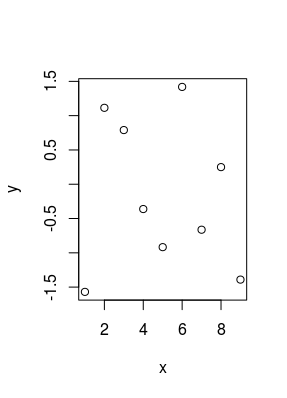
\includegraphics{../assets/sample.png}
    \caption{正态随机数}
\end{figure}

\section{节的标题(仿宋小三号加黑)}
\begin{equation}
\frac{1}{2}
\end{equation}
\subsection{节的标题(仿宋四号加黑)}

符号说明
{\wuhao
\begin{longtable}{p{5cm}p{5cm}}
\caption{符号说明}\\
\hline
项目内容 & 特点\\
\hline
模拟& 同方差\\
\hline
\end{longtable}
}
项目内容

\section{结论}

\printbibliography[heading=chapbib]
%	\end{refsection}
% \end{latex}
% \subsubsection{文献标题}
% 注意到在第一部分文献标题是以 chapter 格式出现,而在第二部分文献标题是以 section 形式出现。本模板提供这两种格式的文献标题,分别通过下面的命令实现
% \begin{latex}
% % chapter 形式的文献标题
% \printbibliography[heading=chapbib]
% % section 形式的文献标题
% \printbibliography[heading=secbib]
% \end{latex}
%\subsection{独立页面}
% 这里的独立页面指的是考核表、任务书,以及外文原文,这类独立页面的特点是不需更改,所以一种生成独立页面的快捷方式便是直接插入 pdf,这可以通过 pdfpages 包实现。这个处理方案非常适合插入外文原文,既不破坏外文原文的格式,也能设置其页眉页脚使其适应主文档(在学校给出的三合一文件的模板中是需要编页码的,但是在毕业论文目标中不需要编页码)。比如用下列代码插入任务书
% \begin{latex}
% \includepdf[fitpaper=true,pages=-,pagecommand={\thispagestyle{empty}},addtotoc={
%		100, alonepage, 1, 《浙江大学本科生毕业论文(设计)任务书》, task
% }]{../assets/official-1-task.pdf}
% \end{latex}
% 需要说明的是,一般从word直接转换后的pdf存在多种编码格式,这时候不能成功插入,我们需要将多种编码格式转换为单一编码格式,在 Ubuntu 下可以这样处理\footnote{参考\href{https://tex.stackexchange.com/questions/106964/could-not-insert-pdf-graphics}{xetex - Could not insert pdf graphics - TeX - LaTeX Stack Exchange}}:
% \begin{shell}
% $ pdftops official-1-task.pdf
% $ epstopdf official-1-task.ps
% \end{shell}
% assets 文件夹中的文件都已经处理过了,可以直接插入到主文档中。
%\subsection{demo}
% demo 文件夹给出了一个示例。
%\section{实现细节}
%\subsection{基本信息}
%    \begin{macrocode}
%<*cls>
\hyphenation{zju-thesis}
\def\zjuthesis{\textsc{zju-thesis}}
\def\version{1.0}
\LoadClass[a4paper,12pt,openany]{book}
%    \end{macrocode}
%\subsection{字体设置}
% 用 xkeyval 的 \texttt{key=value} 格式来设置中文字体。
%    \begin{macrocode}
\RequirePackage{xkeyval}
\newif\ifzju@fang 
\newif\ifzju@hei
\newif\ifzju@blind
\zju@fangfalse
\zju@heifalse
\zju@blindfalse
\RequirePackage{ifthen}
\DeclareOptionX{fangfont}{\def\fangfont{#1}\zju@fangtrue}%
\DeclareOptionX{heifont}{\def\heifont{#1}\zju@heitrue}%
\DeclareOptionX{blind}{\zju@blindtrue}
%\ExecuteOptionsX{fangfont,heifont}
\ProcessOptionsX%
\ifzju@fang\relax\else
    \ClassError{zju-thesis}{%
                    Please specify fang font in option
                    }{}
\fi
\ifzju@hei\relax\else
    \ClassError{zju-thesis}{%
                    Please specify hei font in option
                    }{}        
\fi 
%    \end{macrocode}
% 字体设置
%    \begin{macrocode}
\RequirePackage{xeCJK} 
\RequirePackage{fontspec} 
\xeCJKsetup{AutoFakeBold=1}

\setCJKfamilyfont{fang}{\fangfont}
\setCJKfamilyfont{hei}{\heifont}

\newcommand*{\fang}{\CJKfamily{fang}}
\newcommand*{\hei}{\CJKfamily{hei}}

\setCJKmainfont{\fangfont}
%    \end{macrocode}
% 定义 48 磅黑体,用于 part 的标题:
%	 \begin{macrocode}
\newcommand{\partheifont}{\fontsize{48pt}{\baselineskip}
        \CJKfontspec[AutoFakeBold=false]{\heifont}\bfseries} 
%    \end{macrocode}
% 定义 36 磅仿宋加粗,用于 part 的标题:
%	 \begin{macrocode}
\newcommand{\partfangfont}{\fontsize{36pt}{\baselineskip}
        \CJKfontspec[AutoFakeBold=4]{\fangfont}\bfseries} 
%    \end{macrocode}
% 定义三号仿宋加粗\cs{chap}(一般用在章标题中),以及无加粗的三号仿宋\cs{chap*}(用在封面信息填写)\footnote{带star选项的命令定义参见\href{http://www.tex.ac.uk/FAQ-cmdstar.html}{Commands defined with * options}}。
%	 \begin{macrocode}
%\newcommand{\chap}{\fontsize{16pt}{\baselineskip}\CJKfontspec[AutoFakeBold=4]{\fangfont}\bfseries}
\newcommand{\sanhao}{\fontsize{16pt}{\baselineskip}\selectfont}
\newcommand{\chap}{\@ifstar%
    {\fontsize{16pt}{\baselineskip}\CJKfontspec[AutoFakeBold=false]{\fangfont}\sanhao}
    {\fontsize{16pt}{\baselineskip}\CJKfontspec[AutoFakeBold=4]{\fangfont}\bfseries}}
%    \end{macrocode}
% 类似地,定义小三号仿宋加粗\cs{sect}(一般用在第一层节标题中) 和 无加粗的小三号仿宋\cs{sect*}。
%    \begin{macrocode}
%\newcommand{\sect}{\fontsize{15pt}{\baselineskip}\CJKfontspec[AutoFakeBold=4]{\fangfont}\bfseries} 
\newcommand{\sect}{\@ifstar%
    {\fontsize{15pt}{\baselineskip}\CJKfontspec[AutoFakeBold=false]{\fangfont}} 
    {\fontsize{15pt}{\baselineskip}\CJKfontspec[AutoFakeBold=4]{\fangfont}\bfseries}}
%    \end{macrocode}
% 以及四号仿宋加粗\cs{subsec} 和无加粗版本\cs{subsec*}
%    \begin{macrocode}
%\newcommand{\subsec}{\fontsize{14pt}{\baselineskip}\CJKfontspec[AutoFakeBold=4]{\fangfont}\bfseries}
\newcommand{\subsec}{\@ifstar
    {\fontsize{14pt}{\baselineskip}\CJKfontspec[AutoFakeBold=false]{\fangfont}\bfseries}
    {\fontsize{14pt}{\baselineskip}\CJKfontspec[AutoFakeBold=4]{\fangfont}\bfseries}}
%    \end{macrocode}
% 小四号仿宋(正文字体)     
%    \begin{macrocode}
\newcommand{\xiaosihao}{\fontsize{12pt}{\baselineskip}\CJKfontspec[AutoFakeBold=false]{\fangfont}} 
%    \end{macrocode}
% 五号宋体(表格字体)【暂时用仿宋代替】     
%    \begin{macrocode}
\newcommand{\wuhao}{\fontsize{10.5pt}{\baselineskip}\CJKfontspec[AutoFakeBold=false]{\fangfont}} 
%    \end{macrocode}
% \subsection{设置页边距}
%    \begin{macrocode}
\RequirePackage[left=2.5cm,right=2.0cm,top=2.5cm,bottom=2.0cm]{geometry}
%    \end{macrocode}
% \subsection{设置页眉页脚}
%    \begin{macrocode}

\renewcommand{\title}[2]{\gdef\titleown{#1}\gdef\titlezju{#2}}
\ifzju@blind%
    \renewcommand{\author}[2]{\gdef\name{\relax}\gdef\stuid{\relax}}
    \newcommand{\grade}[2]{\gdef\grade{\relax}\gdef\major{\relax}}
    \newcommand{\school}[1]{\gdef\school{\relax}}
    \newcommand{\mentor}[1]{\gdef\mentor{\relax}}
\else%
    \renewcommand{\author}[2]{\gdef\name{#1}\gdef\stuid{(#2)}}
    \newcommand{\grade}[2]{\gdef\grade{#1}\gdef\major{#2}}
    \newcommand{\school}[1]{\gdef\school{#1}}
    \newcommand{\mentor}[1]{\gdef\mentor{#1}}
\fi
\renewcommand{\date}[1]{\gdef\date{#1}}

\RequirePackage{fancyhdr}
%    \end{macrocode}
% 封面页无页眉页脚
%    \begin{macrocode}
\fancypagestyle{firstpage}{%
	\fancyhf{} % clear fields
	\renewcommand{\headrulewidth}{0pt} % no line
	\renewcommand{\footrulewidth}{0pt} % no line
}
\fancypagestyle{guidepage}{%
	\fancyhf{} % clear fields
	\renewcommand{\headrulewidth}{0.7pt} % no line
	\renewcommand{\footrulewidth}{0pt} % no line
	\fancyhead[R]{\titleown}
}
%    \end{macrocode}
% 正文页面格式,按照学校给出的 word 模板。具体要求如下:\par
%
% \begin{itemize}
%	\item 奇数页右页眉(毕业论文(设计)题目)
%	\item 偶数页左页眉(浙江大学本科生毕业论文(设计))
% \end{itemize}
%    \begin{macrocode}
\fancypagestyle{followingpage}{%
	\fancyhf{} % clear fields
	% thesis title on the right header on the odd-number pages
	\fancyhead[RO]{\titleown}
	\fancyhead[LE]{\titlezju}
	% official name on the left header of the even-number pages	
	% page number on the center footer of all pages
	\fancyfoot[C]{\thepage}
	\renewcommand{\headrulewidth}{0.7pt}
	\renewcommand{\footrulewidth}{0pt}
}

\AtBeginDocument{\thispagestyle{firstpage}}
\AtBeginDocument{\assignpagestyle{\chapter}{followingpage}}
%\AtBeginDocument{\assignpagestyle{\guide}{followingpage}}
\pagestyle{followingpage}
%    \end{macrocode}
% \subsection{图表格式}
% 图表格式的具体要求为
%
% \begin{itemize}
% \item 图标题在图下面,表标题在表上面;
% \item 图、表标题均采用五号宋体加粗;
% \item 表格中文字采用5号宋体,行距为单倍行间距;
% \item 图、表与下文空一行。
% \end{itemize}
%    \begin{macrocode}
\renewcommand{\figurename}{图}
\renewcommand{\tablename}{表}
\RequirePackage[labelfont=bf,tableposition=top]{caption}
\RequirePackage{float}
%    \end{macrocode}
% \subsection{节标题设置}
% 标题样式的具体要求为
%
% \begin{itemize}
%	\item 章标题:三号仿宋加黑
%	\item 第一层节标题:小三号仿宋加黑
%	\item 第二层节标题:四号仿宋加黑
%	\item 第三层节标题:四号仿宋加黑(需要说明的是,此处 Word 模板中 1.1 节和 1.2 节格式要求不同,怀疑是 typo。)
% \end{itemize}
% 
%    \begin{macrocode}
\RequirePackage{titlesec}
\newcommand{\chapterbreak}{\clearpage}

\renewcommand\section{\@startsection
	{section}{1}{\z@}%name, level, indent
	{-3.5ex \@plus -1ex \@minus -.2ex}%             beforeskip
	{2.3ex \@plus.2ex}%            afterskip
	{\sect}}% style

\renewcommand\subsection{\@startsection
	{subsection}{2}{\z@}%name, level, indent
	{-3.25ex\@plus -1ex \@minus -.2ex}%             beforeskip
	{1.5ex \@plus .2ex}%            afterskip
	{\subsec}}% style

\renewcommand\subsubsection{\@startsection
	{subsubsection}{3}{\z@}%name, level, indent
	{-3.25ex\@plus -1ex \@minus -.2ex}%             beforeskip
	{1.5ex \@plus .2ex}%            afterskip
	{\subsec}}% style
%    \end{macrocode}
% \subsection{文献引用}
% 提供三种文献引用的格式 \cs{cite},\cs{parencite} 以及 \cs{textcite},并且默认用蓝色高亮(是否需要?)
%    \begin{macrocode}
\RequirePackage{csquotes}
\RequirePackage{xcolor} % DO NOT forget
\RequirePackage[backend=biber,citestyle=authoryear,sortcites=true,natbib]{biblatex}
%% set citation color as blue
%\renewcommand\nametitledelim{\ifin{textcite}{\addspace}{\addspace\addcomma}}
\DeclareCiteCommand{\cite}
  {\color{blue}\usebibmacro{prenote}}%
  {\usebibmacro{citeindex}%
   \usebibmacro{cite}}
  {\multicitedelim}
  {\usebibmacro{postnote}}
\DeclareCiteCommand{\parencite}[\mkcolorbibparens]
  {\usebibmacro{prenote}}%
  {\usebibmacro{citeindex}%
   \usebibmacro{cite}}
  {\multicitedelim}
  {\usebibmacro{postnote}}
\DeclareCiteCommand{\textcite}
  {\color{blue}
	  \renewcommand*\nameyeardelim{\addspace}%
	  \boolfalse{cbx:parens}%
   \renewcommand*{\finalnamedelim}{% <---- this is new
     \ifnumgreater{\value{liststop}}{2}{\finalandcomma}{}%
     \addspace\bibstring{and}\space}}
  {\usebibmacro{citeindex}%
   \iffirstcitekey
     {\setcounter{textcitetotal}{1}}
     {\stepcounter{textcitetotal}%
      \textcitedelim}%
   \usebibmacro{textcite}}
  {\ifbool{cbx:parens}
     {\bibcloseparen\global\boolfalse{cbx:parens}}
     {}}
  {\usebibmacro{textcite:postnote}}
\makeatletter
\newrobustcmd{\mkcolorbibparens}[1]{%
	\begingroup
	\color{blue}%
	\blx@blxinit
	\blx@setsfcodes
	\bibopenparen#1\bibcloseparen
	\endgroup}
\makeatother
%\patchcmd{\thebibliography}{\chapter*}{\section*}{}{}
\bibliography{ref.bib}
\addbibresource{ref.bib}
%\defbibheading{secbib}[]{% rename and change style to section
%    \end{macrocode}
% 定义两种格式的参考文献标题,一种是以 chapter 形式出现,如第一部分,第二种是以 section 形式出现,如第二部分。
%    \begin{macrocode}
\defbibheading{chapbib}[参考文献]{%
  \chapter{#1}%
  \markboth{#1}{#1}}
\defbibheading{secbib}[参考文献]{%
  \section{#1}%
  \markboth{#1}{#1}}
%    \end{macrocode}
% \subsection{章标题设置}
% \subsubsection{基本设置}
% 首先设置 chapter 和 part 的中文格式,并用 \cs{counterwithin} 使章节编号独立于每个 part。
%    \begin{macrocode}
\RequirePackage{zhnumber}
\RequirePackage{chngcntr}
\counterwithin{chapter}{part}
\counterwithin*{page}{part}

\AtBeginDocument{\assignpagestyle{\part}{firstpage}}
\renewcommand\thepart{第\zhnum{part}部分} 
\renewcommand{\partname}{}
%\titleformat{\part}[display]{\partheifont\normalfont\Huge}{{\thepart}}{72pt}{\Huge}
%    \end{macrocode}
%   \subsubsection{独立样式(deparcated)}
% Update:因为第二部分直接用\cs{includepdf} 插入到主文档中,所以该功能移除。所以直接设置第一部分的样式就好了。
%    \begin{macrocode}
\renewcommand{\thechapter}{\arabic{chapter}}
\renewcommand{\thesection}{\arabic{chapter}.\arabic{section}}
\titleformat{\chapter}{\chap}{\thechapter}{1em}{}
\titlespacing*{\chapter}{0pt}{0pt}{2.3ex plus .2ex}

\makeatletter
\def\@part[#1]#2{%
    \ifnum \c@secnumdepth >-2\relax
        \refstepcounter{part}%
        \addcontentsline{toc}{part}{\thepart\hspace{1em}#1}%
    \else
        \addcontentsline{toc}{part}{#1}%
    \fi
    \markboth{}{}%
    {\centering
    \interlinepenalty \@M
    \normalfont
    \ifnum \c@secnumdepth >-2\relax
    {\partheifont \partname\nobreakspace\thepart}
    \par
    \vskip 72\p@
    \fi
    {\partfangfont #2}\par}%
    \@endpart}
\makeatother
%    \end{macrocode}
% 第二部分三合一文件需要中文编号,但第一部分正文不需要中文编号。且对第一个 part 需要设置左对齐的 chapter,对第二个 part 设置居中的 chapter 格式。所以我们对这两个部分的 chapter 单独设置格式。因为 \cs{titlesec} 可以放在任意地方,因此最简单的方法便是在 tex 文档中的每个 part 部分手动设置 \cs{titlesec},但还是想将其封装到 .cls 文件中。想法是自定义依赖于具体 part 编号的 \cs{mypart} 命令,然后将该命令插入到对应的 part 之后。对于插入的位置,我选择重定义 \cs{part},将 \cs{mypart} 包含其中。
% \DescribeMacro{\mypart}
%    \begin{macrocode}
%\newcommand{\mypart}{%
% \ifthenelse{\arabic{part}=0}{% why zero and not one
% %\ifthenelse{\equal{\thepart}{第一部分}}{%
%     \renewcommand{\thechapter}{\arabic{chapter}}
%     \renewcommand{\thesection}{\arabic{chapter}.\arabic{section}}
%     \titleformat{\chapter}{\chap}{\thechapter}{1em}{}
%     \titlespacing*{\chapter}{0pt}{0pt}{2.3ex plus .2ex}
% }{%
% 	\renewcommand{\chaptername}{}
%     \renewcommand\thechapter{\zhnum{chapter}、} 
%     \renewcommand{\thesection}{\arabic{section}}
%     \titleformat{\chapter}[hang]{\centering\chap}{\chaptertitlename\ \thechapter}{0pt}{}
%     \titlespacing*{\chapter}{0pt}{0pt}{2.3ex plus .2ex}
%  }
% }
% \makeatletter
% \def\@part[#1]#2{%
%     \ifnum \c@secnumdepth >-2\relax
%         \refstepcounter{part}%
%         \addcontentsline{toc}{part}{\thepart\hspace{1em}#1}%
%     \else
%         \addcontentsline{toc}{part}{#1}%
%     \fi
%     \markboth{}{}%
%     {\centering
%     \interlinepenalty \@M
%     \normalfont
%     \ifnum \c@secnumdepth >-2\relax
%     {\partheifont \partname\nobreakspace\thepart}
%     \par
%     \vskip 72\p@
%     \fi
%     {\partfangfont #2}\par}%
%     \@endpart}
% \makeatother

% \makeatletter
% \renewcommand\part{%
%     \if@openright
%         \cleardoublepage
%     \else
%         \clearpage
%     \fi
%     \thispagestyle{empty}%
%     \if@twocolumn
%     \onecolumn
%     \@tempswatrue
%     \else
%     \@tempswafalse
%     \fi
%     \null\vfil\relax\mypart
%     \secdef\@part\@spart} %[WARNING!!!!!!] the location of mypart
% \makeatother

% \makeatletter
% \renewcommand\@endpart{
% \vfil\newpage
% \if@twoside
% \if@openright
% \null
% \thispagestyle{empty}%
% \newpage
% \fi
% \fi
% \if@tempswa
% \twocolumn
% \fi
% }
% \makeatother
% \makeatletter
% \DeclareRobustCommand\@part[#1]#2{%
%     \ifnum \c@secnumdepth >-2\relax
%         \refstepcounter{part}%
%         \addcontentsline{toc}{part}{\thepart\hspace{1em}#1}%
%     \else
%         \addcontentsline{toc}{part}{#1}%
%     \fi
%     \markboth{}{}%
%     {\centering
%     \interlinepenalty \@M
%     \normalfont
%     \ifnum \c@secnumdepth >-2\relax
%     \huge\bfseries \partname\nobreakspace\thepart
%     \par
%     \vskip 20\p@
%     \fi
%     \Huge \bfseries #2\par}%
%     \@endpart}
% \makeatother
%    \end{macrocode}
% 虽然现在能达到目的,但测试代码的时候有几点很困惑,具体为
% \begin{itemize}
% \item \cs{ifthenelse} 中判断条件的设置,起初用 \cs{arbic}\{part\}=1 来判断是否是第一部分(这时还没有用\cs{titleformat}),运行正常;
% \item 当进行 \cs{titleformat} 设置时,不能达到预期效果,则尝试使用 \cs{equal}\{\cs{part}\}\{第一部分\} 来判断是否为第一部分,运行正常,但是此时 part 的样式不对;
% \item \cs{mypart} 放置的位置也有区别,先后试了 \cs{part} 的末尾,\cs{@part} 和 \cs{@endpart} 中的位置,都不能达到效果;
% \item 最后将 \cs{mypart} 放置当前位置,运行正常,但第一部分和第二部分是反的,当将判定条件修改为当前位置,得到预期效果。
% \item 我的猜想是因为\cs{mypart} 放在了 \cs{@part} 之前,所以可能计数器(或者其它量)还未完成赋值就运行 \cs{mypart},但又不能放在最后,否则 part 的样式出现问题——标题和标签跨页,似乎是标题参数由于\cs{mypart}的存在未能正确传递。
% \end{itemize}
%    \begin{macrocode}
%\renewcommand{\chaptername}{}

%\renewcommand\thechapter{\zhnum{chapter}、} 

%\renewcommand{\thechapter}{\arabic{chapter}} 
%\renewcommand\thesection{\arabic{section}}
%\titleformat{\chapter}[hang]{\centering\chap}{\chaptertitlename\ \thechapter}{0pt}{}
%\titlespacing*{\chapter}{0pt}{0pt}{40pt}
%\titleformat{\section}{\sect}{\sectiontitlename\ \thesection}{1em}{}
%\titleformat{\subsection}{\sihao}{\thesubsection}{}{}
%\titleformat{\subsubsection}{\sihao}{\thesubsubsection}{}{}
%    \end{macrocode}
% 此处为 TeXLive 2015 在 Ubuntu 上的一个 bug,section 编号会消失,在 Window 下曾做过测试,不会消失,下面的命令能够解决这个历史性 bug,这个 bug 在新版 TeXLive 中 已经改过来了。参考\href{https://tex.stackexchange.com/questions/299969/titlesec-loss-of-section-numbering-with-the-new-update-2016-03-15}{texlive - titlesec: loss of section numbering with the new update (2016/03/15) - TeX - LaTeX Stack Exchange}
%    \begin{macrocode}
%% fix section numbering bug
\RequirePackage{etoolbox}%
\makeatletter
\patchcmd{\ttlh@hang}{\parindent\z@}{\parindent\z@\leavevmode}{}{}%
\patchcmd{\ttlh@hang}{\noindent}{}{}{}%
\makeatother
%    \end{macrocode}
% 设置目录及标题深度(似乎不需要)
%    \begin{macrocode}
\setcounter{tocdepth}{6}
\setcounter{secnumdepth}{6}
\RequirePackage{titletoc}
%    \end{macrocode}
% 设置任务书及考核表在目录中的标题格式
%    \begin{macrocode}

\titleclass{\alonepage}{straight}[\part]
\newcounter{alonepage}
\titleclass{\contabpage}{straight}[\part]
\newcounter{contabpage}
\contentsmargin{0pt}
%    \end{macrocode}
% 目录格式设定,注意到学校给的模板的目录中的标题是左对齐的,但\cs{titletoc} 会使得每一层目录有缩进,即使通过\cs{titlecontents} 设置 left 为 0pc,所以最后用了 \cs{makebox} 使标题左对齐,注意使用时要考虑 label 的宽度,所以设置先设置 2pc 的left,然后用\cs{hspace*\{-2pc\}} 补回来,其中的 2pc 宽度便是留给 label的。\footnote{此处参考\href{https://tex.stackexchange.com/questions/96265/text-alignment-issue-in-custom-table-of-contents?rq=1}{Text alignment issue in custom Table of Contents - TeX - LaTeX Stack Exchange}。}
%    \begin{macrocode}
\titlecontents{alonepage}[0pc]{}{}{}{}
\titlecontents{contabpage}[0pc]{}{}{}{\titlerule*[1pc]{.}\thecontentspage}
\titlecontents{part}[0pc]{\chap\bfseries}{}{}{}
\titlecontents{chapter}[0pc]{\addvspace{0pt}\hspace*{0pc}}{\thecontentslabel}{}{
	\titlerule*[1pc]{.}\thecontentspage}%[\addvspace{3pt}]
%\titlecontents{section}[1.8pc]{\addvspace{3pt}\bfseries}{
%	\thecontentslabel }{}{\titlerule*[1pc]{.}\thecontentspage}
\titlecontents{section}[2pc]{}{\makebox[0pt][l]{\hspace*{-2pc}\thecontentslabel}}{}{\titlerule*[1pc]{.}\thecontentspage}
\titlecontents{subsection}[3pc]{}{\makebox[0pt][l]{\hspace*{-3pc}\thecontentslabel}}{
	}{\titlerule*[1pc]{.} \thecontentspage}
\titlecontents{subsubsection}[4pc]{\small}{\makebox[0pt][l]{\hspace{-4pc}\thecontentslabel}}{
	}{\titlerule*[1pc]{.} \thecontentspage}

%\titlecontents{subsection}[2pc]{}{\thecontentslabel}{
%	}{\titlerule*[1pc]{.} \thecontentspage}
%\titlecontents{subsubsection}[3pc]{\small}{\thecontentslabel}{
%	}{\titlerule*[1pc]{.} \thecontentspage}
%    \end{macrocode}
% \subsection{目录页设置}
% 目录页的 top margin 太大,适当缩小。\footnote{参考\href{https://tex.stackexchange.com/questions/62125/how-to-remove-top-margin-above-tableofcontents}{spacing - How to remove top margin above tableofcontents - TeX - LaTeX Stack Exchange}}
%    \begin{macrocode}

\makeatletter
\let\oldtableofcontents\tableofcontents
\renewcommand{\tableofcontents}{\begingroup%
  \patchcmd{\@makeschapterhead}% <cmd>
    {\vspace*{50\p@}}% <search>
    {}% <replace>
    {}{}% <success><failure>
  \oldtableofcontents%
  \endgroup%
}
\makeatother
\renewcommand{\contentsname}{{\centerline{目\hspace*{1em}录}}}
%    \end{macrocode}
% \subsection{行距设置}
%    \begin{macrocode}
\RequirePackage{setspace}
\spacing{1.5}
%    \end{macrocode}
% \subsection{等式编号独立 (deparcated)}
% 在写三合一文件时,每部分的公式编号是独立的,不过在正式论文中应当取消这个设定。\href{https://github.com/szcf-weiya/zju-thesis/issues/4}{Issue \#4}
%    \begin{macrocode}
%\renewcommand{\theequation}{\arabic{equation}}
%    \end{macrocode}
% \subsection{首行缩进}
% 虽然默认段落的首行会缩进,但每节的第一段并没有首行缩进。
%    \begin{macrocode}
\RequirePackage{indentfirst}
%    \end{macrocode}

% \subsection{生成封面}
%  三合一文件需要一个封面,自定义命令 \cs{makecoverprop} 来生成三合一文件的封面。
% \DescribeMacro{\makecoverprop}
%    \begin{macrocode}
\RequirePackage{graphicx}
\newcommand\hp{\hspace{0.35em}}
\newcommand*{\makecoverprop}
{	
	\begingroup 
	\begin{center}

		\includegraphics[width=0.8\textwidth]{../assets/zju-text.png}
		\\[1.2\baselineskip]
		%\vspace*{0.05\paperheight} % White space at the top of the page
		{\Huge{\hei\bfseries {本\hp 科\hp 生\hp 毕\hp 业\hp 论\hp 文(设\hp 计) \\[0.8\baselineskip]文献综述和开题报告}}}\\[1.2\baselineskip] % Title
		\includegraphics[width=0.35\textwidth]{../assets/zju-xiaohui.jpg}
		\vspace*{3\baselineskip} % Whitespace between 
		\begin{table}[h!]
		  \begin{center}
			\begin{tabular}{ll} 
			\subsec{姓名与学号} & \underline{\makebox[7cm][c]{\name (\stuid)}}  \\[5ex]
			\subsec{指导教师} & \underline{\makebox[7cm][c]{\mentor}}\\[5ex]
			\subsec{年级与专业} & \underline{\makebox[7cm][c]{\grade\major}}\\[5ex]
			\subsec{所在学院} & \underline{\makebox[7cm][c]{\school}}\\[5ex]
			\end{tabular}
		\end{center}
		\end{table}
		\vspace*{1\baselineskip}
	\end{center}
	\vfill
	\endgroup
	\clearpage
}

%    \end{macrocode}
% 不过对于正式论文,需要新的封面,类似 \cs{makecoverprop},定义新的生成封面的命令 \cs{makecover}。注意格式要求
% \begin{itemize}
%   \item “本 科 生 毕 业 论 文(设计)”为黑体,字体大小没有明确要求,为了简便直接使用 \cs{Huge};
%   \item “题目”为三号华文仿宋加黑(华文仿宋和仿宋差别大么?暂时用仿宋代替);
%   \item 个人信息为三号华文仿宋(同上,暂时用华文仿宋代替)。
%   \item 若盲审,则无需填写个人信息(暂时默认非盲审)TODO:添加盲审选项。
% \end{itemize}
% \DescribeMacro{\makecover}
%    \begin{macrocode}
\newcommand*{\makecover}
{	
	\begingroup 
	\begin{center}

		\includegraphics[width=0.8\textwidth]{../assets/zju-text.png}
		\\[1.2\baselineskip]
		%\vspace*{0.05\paperheight} % White space at the top of the page
		{\Huge{\hei\bfseries {本\hp 科\hp 生\hp 毕\hp 业\hp 论\hp 文(设\hp 计)}}}\\[1.2\baselineskip] % Title
		\includegraphics[width=0.32\textwidth]{../assets/zju-xiaohui.jpg}\\[1\baselineskip]
		%\vspace*{3\baselineskip} % Whitespace between 
        \chap{题目}\ \underline{\makebox[11cm][c]{\chap\titleown}} \\[1.8\baselineskip]
		\begin{table}[h!]
		  \begin{center}
			\begin{tabular}{ll}
			\chap{姓名与学号} & \underline{\makebox[7cm][c]{\chap*{\name \stuid}}}  \\[4ex]
			\chap{指导教师} & \underline{\makebox[7cm][c]{\chap*{\mentor}}}\\[4ex]
			\chap{年级与专业} & \underline{\makebox[7cm][c]{\chap*{\grade\major}}}\\[4ex]
			\chap{所在学院} & \underline{\makebox[7cm][c]{\chap*{\school}}}\\[8ex]
            \chap{提交日期} & \underline{\makebox[7cm][c]{\chap*{\date}}}\\[4ex]
			\end{tabular}
		\end{center}
		\end{table}
		\vspace*{1\baselineskip}
	\end{center}
	\vfill
	\endgroup
	\clearpage
}
%    \end{macrocode}
%    \begin{macrocode}
\setcounter{page}{-1}
\RequirePackage{longtable}
\newcommand\file[1]{\textsf{#1}}
%    \end{macrocode}
% 独立页面的插入
%    \begin{macrocode}
\RequirePackage{pdfpages}
%    \end{macrocode}
% \subsection{算法环境}
%    \begin{macrocode}
\RequirePackage[ruled,linesnumbered]{algorithm2e} 
\SetAlgoCaptionSeparator{\quad}
\SetAlgorithmName{算法}{算法}{算法}
%</cls>
%    \end{macrocode}

% \iffalse
%	\begin{macrocode}
%<*sty>
\ProvidesPackage{\jobname}
\RequirePackage{fontspec}
\RequirePackage{hypdoc}
\RequirePackage{array,longtable}
\RequirePackage{xeCJK}
\RequirePackage{listings}
\RequirePackage{xcolor}
\RequirePackage{fancyhdr}
\RequirePackage{etoolbox}
\RequirePackage{newpxtext}
\RequirePackage{newpxmath}
\RequirePackage[
  top=2.5cm, bottom=2.5cm,
  left=4cm, right=2cm,
  headsep=3mm]{geometry}
\definecolor{cred}{rgb}{0.8,0.8,0.8}
\definecolor{cgreen}{rgb}{0,0.4,0}
\definecolor{cdocblue}{rgb}{0,0,0.6}
\definecolor{cdark}{rgb}{0.75,1.0,1.0}
\definecolor{macro}{rgb}{0.5,0,0.35}
\lstdefinestyle{lstStyleBase}{%
   basicstyle=\ttfamily,
   aboveskip=\medskipamount,
   belowskip=\medskipamount,
   lineskip=0pt,
   boxpos=c,
   showlines=false,
   extendedchars=true,
   upquote=true,
   tabsize=2,
   showtabs=false,
   showspaces=false,
   showstringspaces=false,
   numbers=none,
   linewidth=\linewidth,
   xleftmargin=4pt,
   xrightmargin=0pt,
   resetmargins=false,
   breaklines=true,
   breakatwhitespace=false,
   breakindent=0pt,
   breakautoindent=true,
   columns=flexible,
   keepspaces=true,
   gobble=2,
   framesep=3pt,
   rulesep=1pt,
   framerule=1pt,
   backgroundcolor=\color{cdark},
   stringstyle=\color{cred},
   keywordstyle=\color{cdocblue}\bfseries,
   commentstyle=\slshape\color{cgreen}}

\lstdefinestyle{lstStyleShell}{%
   style=lstStyleBase,
   frame=l,
   rulecolor=\color{purple},
   language=bash}

\lstdefinestyle{lstStyleLaTeX}{%
   style=lstStyleBase,
   frame=l,
   rulecolor=\color{violet},
   language=[LaTeX]TeX}

\lstnewenvironment{latex}{\lstset{style=lstStyleLaTeX}}{}
\lstnewenvironment{shell}{\lstset{style=lstStyleShell}}{}
\setCJKmainfont{STFANGSO.TTF}
\setmainfont{Times New Roman}
\patchcmd{\PrintDescribeMacro}{\MacroFont}{\MacroFont\bfseries\color{macro}}{}{}
\renewcommand{\contentsname}{目录}
\RequirePackage{indentfirst}
\RequirePackage{dirtree}
\newcounter{nodeCdepth}
\newenvironment{nodeC}
  {\ifnum\value{nodeCdepth}=0
     \gdef\listfordirtree{}%
     \let\item\nodeCitem
    \fi
    \stepcounter{nodeCdepth}}
  {\addtocounter{nodeCdepth}{-1}%
   \ifnum\value{nodeCdepth}=0
     \expandafter\dirtree\expandafter{\listfordirtree}%
   \fi}
\newcommand{\nodeCitem}[1]{%
  \xdef\listfordirtree{%
    \unexpanded\expandafter{\listfordirtree}%
    .\thenodeCdepth\space\unexpanded{#1}. }%
}
%</sty>
% 	\end{macrocode}
% \fi
% \Finale
\endinput
